\documentclass[11pt,a4paper]{article}
\usepackage[top=3cm, bottom=2cm, left=2cm, right=2cm]{geometry}
\usepackage[utf8]{inputenc}
\usepackage{amsmath, amsfonts, amssymb}
\usepackage{siunitx}
\usepackage[brazil]{babel}
\usepackage{graphicx}
\usepackage[margin=10pt,font={small, it},labelfont=bf, textfont=it]{caption}
\usepackage[dvipsnames, svgnames]{xcolor}
\DeclareCaptionFont{MediumOrchid}{\color[svgnames]{MediumOrchid}}
\usepackage[pdftex]{hyperref}
\usepackage{natbib}
\bibliographystyle{plainnat}
\bibpunct{\textcolor{MediumOrchid}{\textbf{[}}}{\textcolor{MediumOrchid}{\textbf{]}}}{,}{s}{}{}
\usepackage{color}
\usepackage{footnote}
\usepackage{setspace}
\usepackage{booktabs}
\usepackage{multirow}
\usepackage{subfigure}
\usepackage{fancyhdr}
\usepackage{leading}
\usepackage{indentfirst}
\usepackage{wrapfig}
\usepackage{mdframed}
\usepackage{etoolbox}
\usepackage[version=4]{mhchem}
\usepackage{enumitem}
\usepackage{caption}
\usepackage{titlesec}
\usepackage{tcolorbox}
\usepackage{tikz}
\usepackage{LobsterTwo}
\usepackage[T1]{fontenc}
\usepackage{fontspec}
\usepackage{txfonts}
\usepackage[bottom]{footmisc}
\tcbuselibrary{skins,breakable}
\sisetup{output-decimal-marker={.}}

\makeatletter
\def\footnoterule{\kern-3pt\color{MediumOrchid}\hrule\@width0.6\textwidth height 0.8pt\kern2.6pt}
\makeatother

\renewcommand{\footnotelayout}{\itshape\color{MediumOrchid}}

\AtBeginEnvironment{equation}{\fontsize{13}{16}\selectfont}


\titleformat{\section}{\LobsterTwo\huge\color{CarnationPink}}{\thesection.}{1em}{}
\titleformat{\subsection}{\LobsterTwo\huge\color{CarnationPink}}{\thesubsection}{1em}{}
\titleformat{\subsubsection}{\bf\LobsterTwo\Large\color{MediumOrchid}}{\thesubsubsection}{1em}{}


\DeclareCaptionLabelFormat{figuras}{\textcolor{DarkTurquoise}{Figura \arabic{figure}}}
\captionsetup[figure]{labelformat=figuras}

\makeatletter
\renewcommand\tagform@[1]{\maketag@@@{\color{CarnationPink}(#1)}}
\makeatother

\renewcommand{\theequation}{Eq. \arabic{equation}}
\renewcommand{\thefigure}{Fig. \arabic{figure}}
\renewcommand{\thesection}{\textcolor{CarnationPink}{\arabic{section}}}

\setlist[itemize]{label=\textcolor{CarnationPink}{$\blacksquare$}}

\setlist[enumerate]{label=\textcolor{CarnationPink}{\arabic*.}, align=left, leftmargin=1.5cm}


\newcounter{exemplo}

\NewDocumentEnvironment{exemplo}{ O{} }{%
\allowbreak
\setlength{\parindent}{0pt}
  \begin{mdframed}[
  leftline=true,
  topline=false,
  rightline=false,
  bottomline=false,
  linewidth=2pt,
  linecolor=CarnationPink,
  frametitlerule=false,
  frametitlefont=\LobsterTwo\large\color{CarnationPink},
  frametitle={\color{CarnationPink}\LobsterTwo\large #1},
  ]
}{%
  \end{mdframed}
}

\setlength{\fboxsep}{5pt}
\setlength{\fboxrule}{1.5pt}
\usepackage{float}
\renewcommand{\thefootnote}{\alph{footnote}}
\usepackage{url}
\hypersetup{
	colorlinks=true,
	linkcolor=DarkTurquoise,
	filecolor=DarkTurquoise,      
	urlcolor=DarkTurquoise,
	citecolor=DarkTurquoise,
	pdftitle={Especialista em Física da Radioterapia}
}
\pagestyle{fancy}
\fancyhf{}
\renewcommand{\headrulewidth}{0pt}
\rfoot{\color{DarkTurquoise}\thepage \\ \LobsterTwo{\small\textcolor{CarnationPink}{@defDalila}}}

\title{\LobsterTwo\Huge{Radioterapia}}
\author{\LobsterTwo\Large{IMRT e VMAT}\nocite{*}}
\date{\LobsterTwo\textit{Dalila Mendonça}}
\begin{document}
	\maketitle

\thispagestyle{fancy}
\section{Introdução}

	A radioterapia de intensidade modulada (IMRT - \textit{Intensity-modulated radiotherapy}) fornece um controle excepcional com respeito a entrega da dose. A \ref{fig:imrt7campos} mostra um exemplo de um plano de IMRT com 7 campos para um paciente com carcinoma orofaríngeo T3 de cabeça e pescoço. Este caso ilustra a capacidade de modelar a dose em torno dos órgãos de risco próximos (neste caso, a medula e a parótida) enquanto irradia o volume tumoral bruto (GTV) e as regiões nodais com risco de comprometimento com uma dose alta. Este caso também demonstra a técnica de “dose painting” ou “simultaneous integrated boost (boost concomitante)” em que um único plano é usado para fornecer uma dose total de 70 Gy para a doença presente (GTV), enquanto as regiões nodais recebem simultaneamente uma dose de 59.4 Gy ou 54 Gy. Também está disponível a técnica de IMRT chamada de terapia de arco volumétrico modulado (VMAT - \textit{``volumetric modulated arc therapy''})  que possui capacidade de modelagem da dose semelhante à técnica IMRT com campos estáticos.

	\begin{figure}[h]
		\centering
		\fcolorbox{DarkTurquoise}{white}{%
			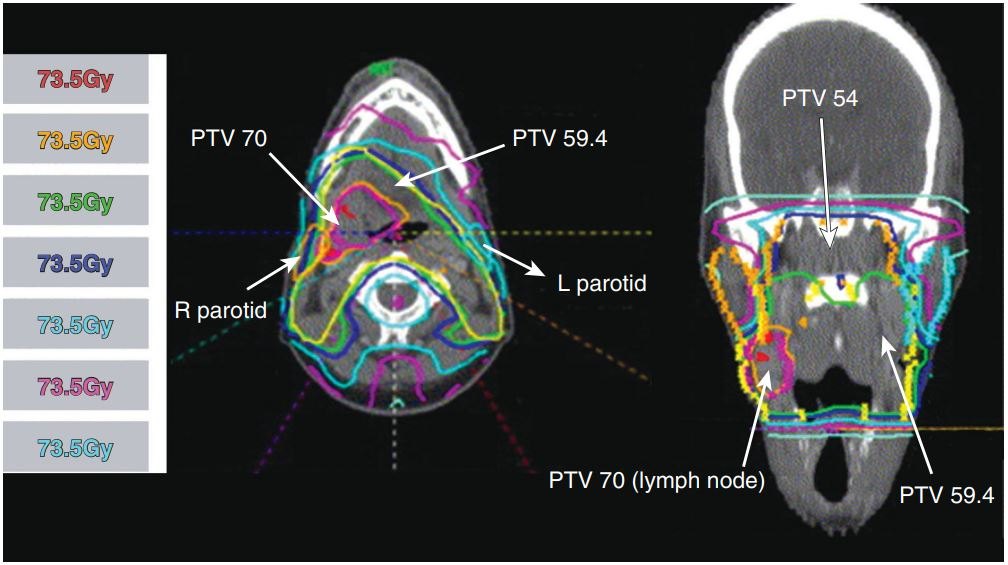
\includegraphics[width=0.7\textwidth]{Imagens/imrt7campos.JPG}
		}%
		\caption{Distribuição de dose para um exemplo de plano IMRT de 7 campos para um paciente com carcinoma de cabeça e pescoço.}
		\label{fig:imrt7campos}
	\end{figure}

	Embora apenas seis ensaios clínicos randomizados tenham sido identificados (três para câncer de mama e três para cabeça e pescoço)(até 2010), no geral, os estudos de caso mostraram um benefício da técnica de IMRT em termos da toxicidade e parâmetros de qualidade de vida. Benefícios específicos foram observados para os seguintes parâmetros: xerostomia\footnote{Xerostomia é o termo médico usado para descrever a sensação de boca seca, que ocorre quando há uma diminuição da produção de saliva na boca.} em casos de cabeça e pescoço, toxicidade retal em casos de próstata, toxicidade gastrointestinal/genitourinária (GI/GU) em casos de câncer uterino e cosmesis\footnote{"Cosmesis" é um termo médico usado para descrever a aparência estética ou o resultado cosmético de um procedimento cirúrgico ou tratamento médico. Refere-se à preocupação estética em relação à cicatrização, reconstrução ou restauração de uma parte do corpo, no caso a mama, para que ela fique o mais natural e harmoniosa possível.} em câncer de mama.

\subsection*{Desenvolvimento Tecnológico}

	Antes de 1994, planos de tratamento ideais eram desenvolvidos usando aberturas do campo, ângulo do colimador, ângulo do gantry, energia do feixe, ponderação do campo e modificadores de feixe como filtros ou compensadores. Alguma modulação básica pode ter sido realizada usando a abordagem \textit{field-in-field}. O indivíduo que estivesse fazendo o planejamento ajustava manualmente os vários parâmetros do plano até que um resultado aceitável, não necessariamente ideal, fosse alcançado. 

	Com o desenvolvimento do colimador multi-lâminas (MLC) e do planejamento inverso, os ajustes passaram de modificações manuais dos parâmetros mecânicos para modificações dos parâmetros relacionados ao alvo e aos órgãos de risco (OARs). Os objetivos e as restrições de dose (constraints) são modificados para produzir um resultado aceitável, mas ainda não necessariamente ideal. Este resultado é obtido por meio do ajuste automático dos vários parâmetros mecânicos pelo algoritmo de otimização em tentativas sequenciais para atender aos objetivos e restrições especificados. As primeiras versões da otimização modificavam a intensidade do feixe apenas modificando a abertura do feixe. Essa técnica foi chamada de radioterapia de intensidade modulada (IMRT). Contudo, foram sendo desenvolvidos sistemas mais modernos que são capazes de otimizar, além da abertura do campo, o ângulo do gantry e o ângulo do colimador.

	O primeiro sistema IMRT disponível comercialmente (Peacock, NOMOS Corp.) foi lançado em 1994 e usava um colimador binário como um dispositivo adicional para ser acoplado em um acelerador linear padrão (linac) com entregas de dose em arco. A intensidade do feixe era modulada ao longo do arco através da abertura e do fechamento das lâminas do colimador. Como as lâminas do colimador descreviam um processo binário, ou estão abertas ou fechadas, a intensidade de um determinado segmento do arco era determinada através da quantidade de tempo que a lâmina ficava aberta durante esse segmento. Depois que um arco era concluído, a mesa era indexada em uma quantidade precisa para tratar o próximo volume ou ``slice (corte)'' do alvo. Este processo era repetido até que todo o alvo fosse coberto. Devido a essa abordagem slice-by-slice, esta técnica é chamada de Tomoterapia serial ou axial e foi esse sistema original que levou ao desenvolvimento da Tomoterapia helicoidal implementada no sistema TomoTherapy Hi-Art (Accuray Systems Inc.). 

	As implementações de IMRT que se seguiram nos linacs tradicionais usaram o MLC padrão do linac para modular o feixe em angulos fixos de gantry e colimador conforme mencionado anteriormente. Esta modulação podia ser feita entregando a dose em vários segmentos fixos onde o feixe é desligado enquanto o MLC está mudando de forma, chamado \textit{step-and-shoot}, ou fazendo com que o MLC mude continuamente de forma enquanto o feixe está constantemente ligado, chamado de \textit{sliding window} ou MLC dinâmico (dMLC), onde a taxa de dose pode ser fixa ou variável. 

	A técnica desenvolvida na sequência utilizava o linac convencional e o MLC para realizar a entrega dinâmica através de um arco,  que é chamada de VMAT. Essa técnica às vezes é referido pelo seu nome de desenvolvimento original, Radioterapia de Arco de Intensidade Modulada  (IMAT - \textit{intensity-modulated arc radiotherapy}) ou por nomes específicos dos fornecedores, como RapidArc (Varian Inc.) ou SmartArc (Philips Inc.).

\section{Nomenclatura das Estruturas}

	Devido à complexidade dos tratamentos IMRT/VMAT, é essencial ter um padrão bem definido para especificar as estruturas e as doses. Esta questão é o tema central de dois relatórios importantes: ICRU-83, \textbf{\textit{`` Volume and Dose Specification for Prescribing, Recording, and Reporting Photon-Beam IMRT''}} e o Sociedade Americana de Oncologia de Radiação (ASTRO) 2009, \textbf{\textit{``Recommendations for Documenting IMRT Treatments''}}. Embora esses relatórios mencionem especificamente o IMRT em seus títulos, eles também se destinam claramente a serem aplicados ao VMAT (que é uma técnica de IMRT né). Esses relatórios defendem o uso de uma nomenclatura padrão para estruturas de planejamento: gross tumor volume (GTV), clinical tumor volume (CTV), internal target volume (ITV), planning target volume (PTV), OAR e planning OAR volume (PRV).


\section{Margens para IMRT/VMAT}

	Outro conceito importante para o planejamento são as margens. A margem especialmente crucial para IMRT/VMAT é aquela usada para expandir o CTV para o PTV. Esta margem afeta diretamente a cobertura do tumor. Regras de margem baseadas na população dos pacientes foram desenvolvidas e estão bem resumidas na Tabela 4.4 do ICRU-83. Uma relação de margem amplamente utilizada é : $2.5 \sum + 0.7 \sigma$, onde $\sum$ e $\sigma$ são as incertezas sistemáticas e aleatórias, respectivamente, no setup do paciente. Deve-se notar, no entanto, que esta relação de margem foi desenvolvida para radioterapia conformacional 3D e pode não ser aplicável para planos de IMRT, que possuem conformidade e gradientes de dose diferentes. 

	Independentemente da regra adequada para definição das margens, deve-se reconhecer que o uso da técnica de IMRT sozinha geralmente não garante uma redução nas margens. O IMRT tem mais impacto em gradientes de dose, o que pode resultar em menos dose nos OARs próximos, mas não afeta a variação do setup para o qual a margem foi projetada para mitigar. A redução da margem é obtida de forma mais adequada por meio do uso de IGRT em vez de IMRT pois uma fórmula de margem como a  $2.5 \sum + 0.7 \sigma$ sugere que a componente sistemática da variabilidade ($\sum$) é aproximadamente 3 vezes mais importante que a a componente aleatória da variabilidade ($\sigma$) e portanto, se as margens devem ser reduzidas, é particularmente importante reduzir a componente sistemática da variabilidade, que pode ser reduzida com a técnica de IGRT.

\section{Report da Dose e Manutenção dos Registros}

	Tanto o ICRU-83 quanto o relatório ASTRO defendem fortemente o report da dose baseado em histograma de dose-volume (DVH) ao invés de reportar a dose para o(s) ponto(s). As especificações de dose pontual não são mais adequadas porque os planos de IMRT/VMAT geralmente têm uma distribuição de dose mais heterogênea dentro do alvo. Se for usada uma prescrição de dose pontual, o alvo, no geral, pode receber mais ou menos dose, dependendo de qual ponto foi selecionado para definir a prescrição. Os reports baseados no DVH também são necessários para comparar um plano específico com os reports publicados de constraints de tecidos normais, como por exemplo os reports do QUANTEC.

	O documento de IMRT da ASTRO 2009 recomenda que a documentação do tratamento IMRT inclua os seguintes documentos:

	\begin{itemize}[label=\textcolor{CarnationPink}{$\star$}]
		\item Diretivas (diretrizes/ orientações) do planejamento de tratamento IMRT;
		\item Resumo do objetivo do tratamento;
		\item Resumo da orientação por imagem;
		\item Resumo do monitoramento de movimentação;
		\item Notas do médico com respeito ao tratamento;
		\item Registro diário do tratamento;
		\item Impressão do plano de tratamento.
		\item Os registros também devem incluir a marca, modelo e versão do software do sistema de planejamento de tratamento usado.
	\end{itemize}

	O relatório da ASTRO recomenda que os registros de tratamento sejam mantidos por pelo menos 5 anos, enquanto o ICRU-83 usa uma recomendação mais rigorosa, porém razoável, de “cinco anos ou o tempo de vida do paciente, o que for mais longo”.
	
\section{Planejamento IMRT/VMAT}

\subsection*{Planejamento Inverso}

	Existe uma vasta literatura sobre planejamento de tratamento inverso IMRT/VMAT e o Capítulo 2 do ICRU-83 apresenta os conceitos básicos de planejamento inverso, funções objetivo e da otimização através de busca de gradiente. Um desenvolvimento no planejamento inverso é a técnica de otimização multicritério (MCO). O conceito básico por trás do MCO é que não se sabe, a priori, qual função objetivo deve ser empregada. Em outras palavras, a importância relativa de vários objetivos para os alvos e OARs é em si uma variável livre. Na prática, as funções objetivo são modificadas de forma iterativa até que um plano clinicamente aceitável seja alcançado. Com o MCO, múltiplas funções objetivo são avaliadas, permitindo uma exploração mais completa ddo espaço de planos de tratamento possíveis. 

\subsection*{Técnicas e Desafios no Planejamento IMRT/VMAT}

	Existe uma grande variedade de técnicas de planejamento em uso para alcançar um bom plano de IMRT. Algumas técnicas práticas incluem:

	\begin{enumerate}
		\item Use um grande número de feixes igualmente espaçados (por exemplo, 7 a 9 feixes coplanares para cabeça e pescoço). Isso elimina a necessidade de otimizar os ângulos do feixe.
		\item Evite feixes paralelos opostos, uma vez que o beamlet ou as aberturas dos feixes opostos estão competindo diretamente em termos da função objetivo.
		\item Use “anéis” ou donuts em volta do volume alvo para aumentar a conformidade da dose ao redor do volume alvo.
		\item Avalie possíveis riscos de colisão entre o paciente e o sistema de entrega do feixe. Isso é especialmente importante para planos VMAT quando são feitos giros de mesa ou quando o isocentro está localizado em uma lesão lateralizada.
	\end{enumerate}

	Em alguns casos, o PTV tem um overlap com um PRV ou mesmo a um OAR. O exemplo clássico é a próstata, que, quando estendida a um PTV, apresenta um overlap com o reto. Uma maneira de lidar com esse overlap é definindo uma sub-região do PTV (por exemplo, $\text{PTV }\cap \text{ Reto}$ para um caso de próstata). Neste caso, um objetivo de DVH é aplicado a esta sub-região para conduzir o planejamento inverso à fornecer uma menor cobertura nessa sub-região. O ICRU-83 sugere esta solução como uma abordagem razoável, mas defende que, quando o plano estiver completo, a dose para todo o volume do PTV ainda deve relatada e não apenas o DVH para o PTV modificado. O ICRU-83 também defende fortemente que a cobertura do PTV não seja comprometida em favor de poupar o OAR, embora esta seja uma decisão clínica e possa não ser possível atingir ambos os objetivos em alguns casos.

	Em comparação com a radioterapia conformada 3D (CRT), as técnicas de IMRT e VMAT tendem a espalhar a região de baixa dose ao redor do paciente de maneiras que nem sempre podem ser previsíveis. A \ref{fig:imrt9campos} ilustra o caso de uma paciente tratando câncer de colo de útero. A preservação do intestino e da bexiga é aparente, mas um “dedo” de dose também é observado no plano de IMRT. É importante avaliar os planos para essas regiões não intencionais de doses altas, e isso é especialmente importante para os planos que envolvem giros de mesa ou entregas não-isocêntricas.

	\begin{figure}[h]
		\centering
		\fcolorbox{DarkTurquoise}{white}{%
			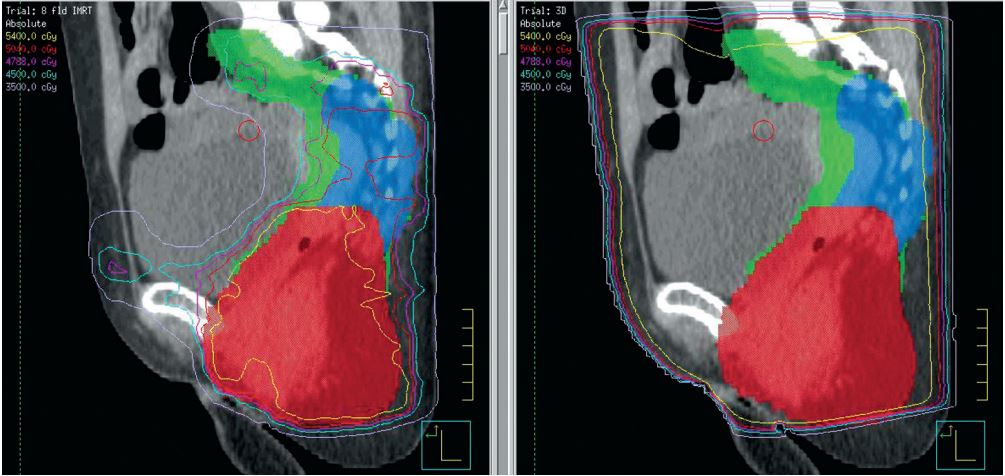
\includegraphics[width=0.8\textwidth]{Imagens/imrt9campos.JPG}
		}%
		\caption{Distribuições de dose para um paciente recebendo tratamento para câncer do colo do útero usando um plano IMRT de 9 campos (à esquerda) e um plano CRT 3D (à direita).}
		\label{fig:imrt9campos}
	\end{figure}

	Em alguns casos, o PTV pode se estender para perto da pele ou até mesmo para o ar (ICRU-83 Seção 5.3.1). Isso apresenta um problema para o planejamento inverso, pois o algoritmo pode tentar aumentar artificialmente a fluência do feixe na região de dose aparentemente baixa próxima da pele ou do ar.  Essa situação pode ser evitada criando um volume de PTV modificado que seja cropado na pele ou mesmo puxado para trás. Este PTV modificado é usado para colocar os objetivos do planejamento inverso. Essa abordagem pode ter como  efeito negativo a subdosagem das regiões superficiais do PTV e/ou eliminar o “Skin-flash” necerrário na pele.

	Outra solução é fazer um sub-volume do PTV na pele e atribuir um peso baixo à função objetivo desse volume (ICRU-83). 

	Outra maneira de direcionar as lâminas do MLC para fora da pele e fornecendo um flash da pele é criando um ``PTV ar'' ou um  ``Fake bolus'' que é uma região que se estende para fora da pele na qual a densidade é substituída para um valor de 1 \unit{g \cdot cm^3}. Esta região recebe um peso muito baixo para o objetivo. Isso serve para direcionar as lâminas do  do MLC para fora do corpo durante a otimização. Após a conclusão da otimização final, o “PTV air” é removido e a dose é recalculada. Entretanto, deve-se ter cuidado com esse método, pois o “PTV air” não representa uma verdadeira estrutura anatômica.


	Em uma nota mais geral, surge a pergunta sobre o que faz um plano de tratamento “bom”. Esta é uma área de investigação ativa para identificar uma métrica significativa para a qualidade do plano. Por exemplo, \citet{WU20111241} desenvolveu a métrica “overlap volume histogram”, que fornece um método de quantificar a preservação do OAR que pode ser obtida com base na população. Outras métricas foram definidas para fins do “desafio do plano”, um concurso anual administrado pela Radiation Oncology Resources Inc. (agora propriedade da Sun Nuclear Inc.) no qual um único caso de planejamento de tratamento é fornecido para vários dosimetristas e físicos. Embora esses resultados ainda não estejam amplamente disponíveis, as pontuações de qualidade parecem não se correlacionar com a experiência, educação ou status de certificação dos planejadores.

	Outra questão prática é: quanto tempo leva (ou deveria) para concluir um plano IMRT ou VMAT? Esta questão foi parcialmente abordada em uma pesquisa multi-institucional de 2009 sobre práticas de IMRT. Os autores descobriram que a resposta dependia de qual sistema de planejamento estava sendo usado, mas concluíram que os casos de cabeça e pescoço exigiam uma média de 30 horas no total (11 horas para planejamento), casos de pulmão 15 horas (planejamento de 8 horas) e casos de próstata 14 horas (planejamento de 6 horas).
	
\section{Entrega e QA}

	Existem muitos métodos diferentes para fornecer tratamentos IMRT e VMAT e cada um tem considerações especiais. Isso inclui tempo de entrega, tempo de beam on,  velocidades mínima e máxima do gantry, taxas de dose mínima e máxima, problemas de colisão, política de aquisição  de imagens, procedimento de entrega interrompido e gerenciamento de movimento. Como muitos dos segmentos usados na IMRT são muito pequenos, pequenas alterações no tamanho da abertura podem afetar significativamente a dose administrada. Devido a esses problemas, é necessário um comissionamento e controle de qualidade de equipamentos mais rigorosos no que diz respeito a IMRT/VMAT. Por exemplo, as tolerâncias de controle de qualidade no AAPM TG-142 são diferentes para uma máquina que executa IMRT e outra que não executa. Algumas informações e ferramentas importantes para validar o desempenho do IMRT podem ser encontradas em AAPM TG-119 (incluindo planos de teste de verificação que podem ser baixados). Phantoms de teste antropomórficos do IROC (anteriormente RPC) também são uma ferramenta de verificação valiosa.


\bibliography{ref.bib}
\end{document}